\documentclass[tikz,border=12pt]{standalone}
\usepackage[no-math]{fontspec}
\usepackage{xeCJK}
\usepackage[UTF8,fontset=none]{ctex}
\usepackage{tikz}
\usetikzlibrary{arrows.meta,positioning,fit,calc,shapes.geometric,backgrounds}

\IfFontExistsTF{Times New Roman}{\setmainfont{Times New Roman}}{\setmainfont{TeX Gyre Termes}}
\IfFontExistsTF{Kaiti TC}{\setCJKmainfont[AutoFakeBold=3]{Kaiti TC}}
  {\IfFontExistsTF{Songti TC}{\setCJKmainfont[AutoFakeBold=3]{Songti TC}}
    {\setCJKmainfont{PingFang TC}}}

% thesis_colors.tex ─ 論文統一 TikZ 色票定義
% 在每個 standalone 圖的 preamble 以 % thesis_colors.tex ─ 論文統一 TikZ 色票定義
% 在每個 standalone 圖的 preamble 以 % thesis_colors.tex ─ 論文統一 TikZ 色票定義
% 在每個 standalone 圖的 preamble 以 \input{thesis_colors.tex} 引入

\definecolor{thesisBlue}{RGB}{43,108,176}      % 訓練集、主箭頭、主色
\definecolor{thesisAmber}{RGB}{201,140,30}     % 驗證集、次要強調
\definecolor{thesisCrimson}{RGB}{155,35,53}    % 測試集、警示
\definecolor{thesisTeal}{RGB}{74,157,143}      % 節點類型 1（電子零組件）
\definecolor{thesisForest}{RGB}{45,122,79}     % 節點類型 2（光電及I/O）、LSTM Update
\definecolor{thesisSand}{RGB}{194,168,120}     % 節點類型 3（半導體）
\definecolor{thesisDark}{RGB}{45,55,72}        % 框線、文字、主箭頭
\definecolor{thesisLight}{RGB}{237,242,247}    % 淡背景、節點填色
\definecolor{thesisPurple}{RGB}{107,70,193}    % GAT 第二注意力頭
\definecolor{thesisMidGray}{RGB}{130,145,160}  % 次要線段、虛線
 引入

\definecolor{thesisBlue}{RGB}{43,108,176}      % 訓練集、主箭頭、主色
\definecolor{thesisAmber}{RGB}{201,140,30}     % 驗證集、次要強調
\definecolor{thesisCrimson}{RGB}{155,35,53}    % 測試集、警示
\definecolor{thesisTeal}{RGB}{74,157,143}      % 節點類型 1（電子零組件）
\definecolor{thesisForest}{RGB}{45,122,79}     % 節點類型 2（光電及I/O）、LSTM Update
\definecolor{thesisSand}{RGB}{194,168,120}     % 節點類型 3（半導體）
\definecolor{thesisDark}{RGB}{45,55,72}        % 框線、文字、主箭頭
\definecolor{thesisLight}{RGB}{237,242,247}    % 淡背景、節點填色
\definecolor{thesisPurple}{RGB}{107,70,193}    % GAT 第二注意力頭
\definecolor{thesisMidGray}{RGB}{130,145,160}  % 次要線段、虛線
 引入

\definecolor{thesisBlue}{RGB}{43,108,176}      % 訓練集、主箭頭、主色
\definecolor{thesisAmber}{RGB}{201,140,30}     % 驗證集、次要強調
\definecolor{thesisCrimson}{RGB}{155,35,53}    % 測試集、警示
\definecolor{thesisTeal}{RGB}{74,157,143}      % 節點類型 1（電子零組件）
\definecolor{thesisForest}{RGB}{45,122,79}     % 節點類型 2（光電及I/O）、LSTM Update
\definecolor{thesisSand}{RGB}{194,168,120}     % 節點類型 3（半導體）
\definecolor{thesisDark}{RGB}{45,55,72}        % 框線、文字、主箭頭
\definecolor{thesisLight}{RGB}{237,242,247}    % 淡背景、節點填色
\definecolor{thesisPurple}{RGB}{107,70,193}    % GAT 第二注意力頭
\definecolor{thesisMidGray}{RGB}{130,145,160}  % 次要線段、虛線


\begin{document}
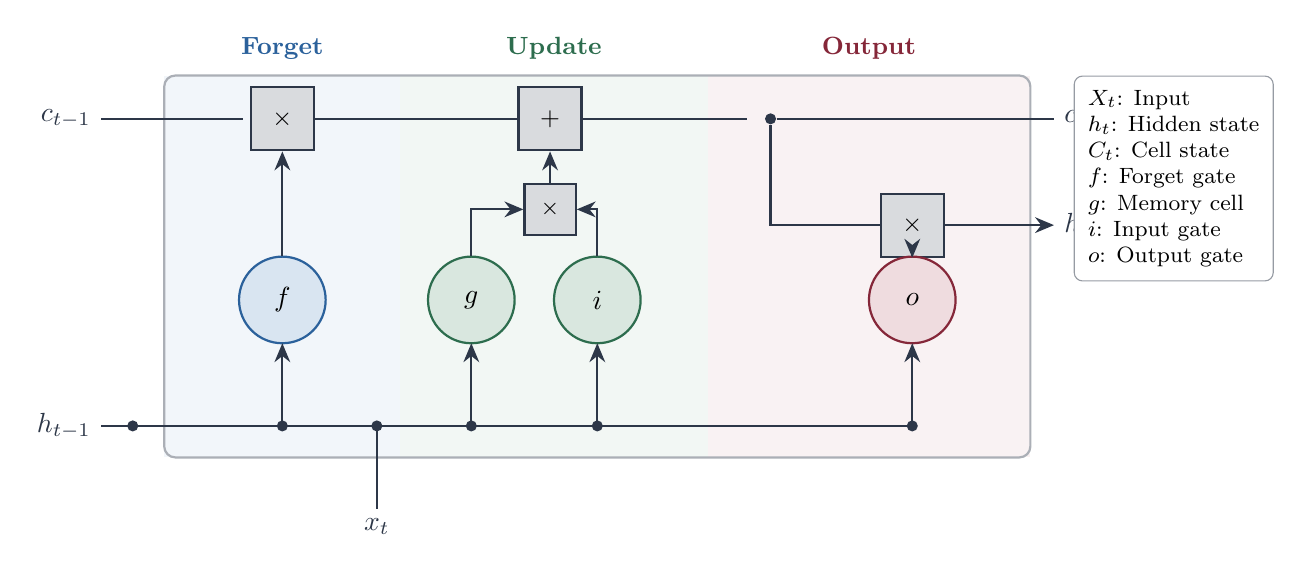
\begin{tikzpicture}[
  % ── operation squares on cell-state line ──
  cellop/.style={draw=thesisDark, fill=thesisDark!18, rectangle,
                 minimum size=8mm, thick, inner sep=1pt, font=\small\bfseries},
  % ── gate circles ──
  fgate/.style={circle, draw=thesisBlue!80!thesisDark, fill=thesisBlue!18,
                thick, minimum size=11mm, font=\normalsize\bfseries},
  ugate/.style={circle, draw=thesisForest!80!thesisDark, fill=thesisForest!18,
                thick, minimum size=11mm, font=\normalsize\bfseries},
  ogate/.style={circle, draw=thesisCrimson!80!thesisDark, fill=thesisCrimson!16,
                thick, minimum size=11mm, font=\normalsize\bfseries},
  % ── arrows ──
  arr/.style={-{Stealth[length=2.4mm,width=2mm]}, thick, thesisDark},
  wire/.style={thick, thesisDark},
  % ── misc ──
  jdot/.style={fill=thesisDark, circle, minimum size=4pt, inner sep=0},
]

%% ─── coordinate helpers ────────────────────────────────────────
% Cell state line  y = 3.2
% Gate row y        = 0.9
% Input wire y      = -0.7
% x positions: L_in=-.5 | ×f=1.8 | +u=5.2 | junction=8.0 | ×o=9.8 | R_out=11.6
% x positions gates: f=1.8 | g=4.2 | i=5.8 | o=9.8

\def\cy{3.2}    % cell-state y
\def\gy{0.9}    % gate y
\def\iy{-0.7}   % input wire y

%% ─── 1. Cell-state wire c_{t-1} → ×f → +u → junction → c_t ───
\draw[wire] (-0.5,\cy) node[left]{$c_{t-1}$} -- (1.3,\cy);
\node[cellop] (Xf) at (1.8,\cy) {$\times$};
\draw[wire] (Xf.east) -- (4.8,\cy);
\node[cellop] (Pu) at (5.2,\cy) {$+$};
\draw[wire] (Pu.east) -- (7.7,\cy);
\node[jdot]  (Jct) at (8.0,\cy) {};   % junction
\draw[wire] (Jct) -- (11.6,\cy) node[right]{$c_t$};

%% ─── 2. Output path: junction → ×o → h_t ─────────────────────
\node[cellop] (Xo) at (9.8,1.85) {$\times$};
% junction → down then right to ×o
\draw[wire] (Jct.south) -- (8.0, 1.85) -- (Xo.west);
% ×o output → h_t
\draw[arr]  (Xo.east)   -- (11.6,1.85) node[right]{$h_t$};

%% ─── 3. Gate circles ───────────────────────────────────────────
\node[fgate] (f) at (1.8,\gy) {$f$};
\node[ugate] (g) at (4.2,\gy) {$g$};
\node[ugate] (i) at (5.8,\gy) {$i$};
\node[ogate] (o) at (9.8,\gy) {$o$};

%% ─── 4. Gate → cell-state connections ─────────────────────────
% f → ×f
\draw[arr] (f.north) -- (Xf.south);

% g and i → intermediate ⊗ → +u
\node[cellop, minimum size=6.5mm, font=\footnotesize] (Xgi) at (5.2,2.05) {$\times$};
\draw[arr] (g.north) -- (4.2,2.05) -- (Xgi.west);
\draw[arr] (i.north) -- (5.8,2.05) -- (Xgi.east);
\draw[arr] (Xgi.north) -- (Pu.south);

% o → ×o
\draw[arr] (o.north) -- (Xo.south);

%% ─── 5. Input wire (h_{t-1} and x_t) ──────────────────────────
% h_{t-1} enters from left on horizontal wire at y=\iy
\draw[wire] (-0.5,\iy) node[left]{$h_{t-1}$} -- (9.8,\iy);
% x_t enters from bottom at x=3.0
\draw[wire] (3.0,-1.75) node[below]{$x_t$} -- (3.0,\iy);
\node[jdot] (Jinput) at (3.0,\iy) {};

% junction dot on h_{t-1} line before x_t join
\node[jdot] (Jh) at (-0.1,\iy) {};  % just the entry point

% Feed from input wire to each gate (vertical arrows up)
\foreach \gx/\gt in {1.8/f, 4.2/g, 5.8/i, 9.8/o}{
  \node[jdot] at (\gx,\iy) {};
  \draw[arr] (\gx,\iy) -- (\gx,\gy-0.55);
}

%% ─── 6. Section labels & subtle backgrounds ────────────────────
% Section shading in background
\begin{pgfonlayer}{background}
  \fill[thesisBlue!6]    (0.3, -1.1) rectangle (3.3, 3.75);   % Forget
  \fill[thesisForest!6]  (3.3, -1.1) rectangle (7.2, 3.75);   % Update
  \fill[thesisCrimson!6] (7.2, -1.1) rectangle (11.3,3.75);   % Output
  % outer border
  \draw[thesisDark!40, rounded corners=4pt, thick]
        (0.3,-1.1) rectangle (11.3,3.75);
\end{pgfonlayer}

% Section titles
\node[font=\small\bfseries, thesisBlue!80!thesisDark]
      at (1.8, 4.1) {Forget};
\node[font=\small\bfseries, thesisForest!80!thesisDark]
      at (5.25,4.1) {Update};
\node[font=\small\bfseries, thesisCrimson!80!thesisDark]
      at (9.25,4.1) {Output};

%% ─── 7. Legend box ──────────────────────────────────────────────
\node[draw=thesisDark!50, rounded corners=3pt, fill=white, inner sep=5pt,
      font=\footnotesize, align=left, anchor=north west]
  at (11.85, 3.75)
  {$X_t$: Input\\$h_t$: Hidden state\\$C_t$: Cell state\\
   $f$: Forget gate\\$g$: Memory cell\\$i$: Input gate\\$o$: Output gate};

\end{tikzpicture}
\end{document}
